\section{Survey Analysis}
\label{research:SurveyAnalysis}
With 41 respondents to my survey thus far I have my response goal and gained a lot of useful information. Throughout this analysis I will show the data I gathered and explain the learnings I have gained from this. Bear in mind each questionable was optional so there may be a smaller numbers of Reponses especially (as I predicted) around the longer format questions 

\subsection*{Q1: Which user group best fits your occuopation?}
\begin{figure}[H]
    \centering
    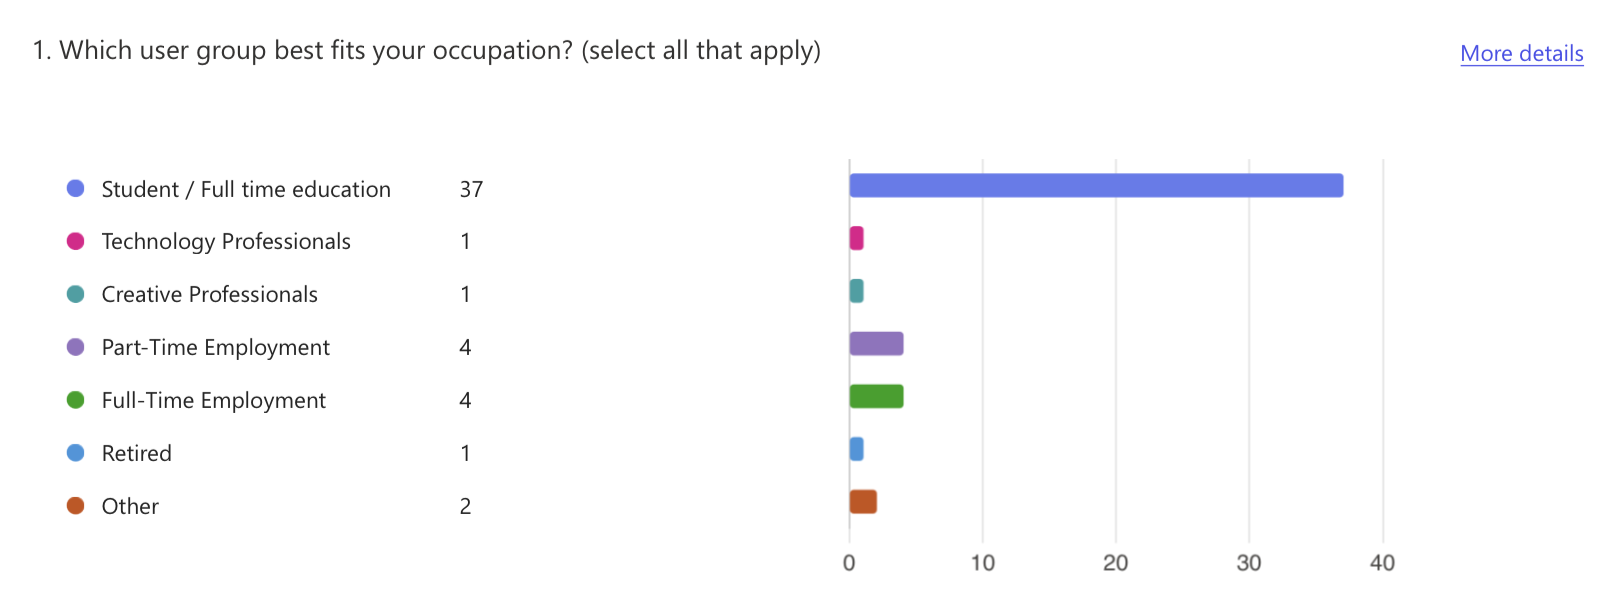
\includegraphics[width=0.8\textwidth]{Research/15_SurveyAnalysis/media/q1.png}
    \caption{Q1 responses}
\end{figure}

From this first question I aimed to ascertain the demographic answering my survey, as expected the vast majority of respondents were students (who are also my target audience) although I did gather a couple of very insightful responses from professionals. I chose the categories above to try and understand if (other than students) there was a link between those in technical industries and those who use more advanced note taking platforms such as obsidian(and inversely those in creative industries using more free-flowing tools such as notability), though in hindsight this question could have been better framed as a few of the respondents were (in my mind at least) classified as technological professionals but didn’t self-select (of the 'other' category of response both stated classification as a technological professional). Fortunately this made little impact to my data set (with this question being mostly auxiliary to my main goals) but is definitely a learning point for next time

\subsection*{Q2: How frequently do you find yourself utilising note taking opportunities?}
\begin{figure}[H]
    \centering
    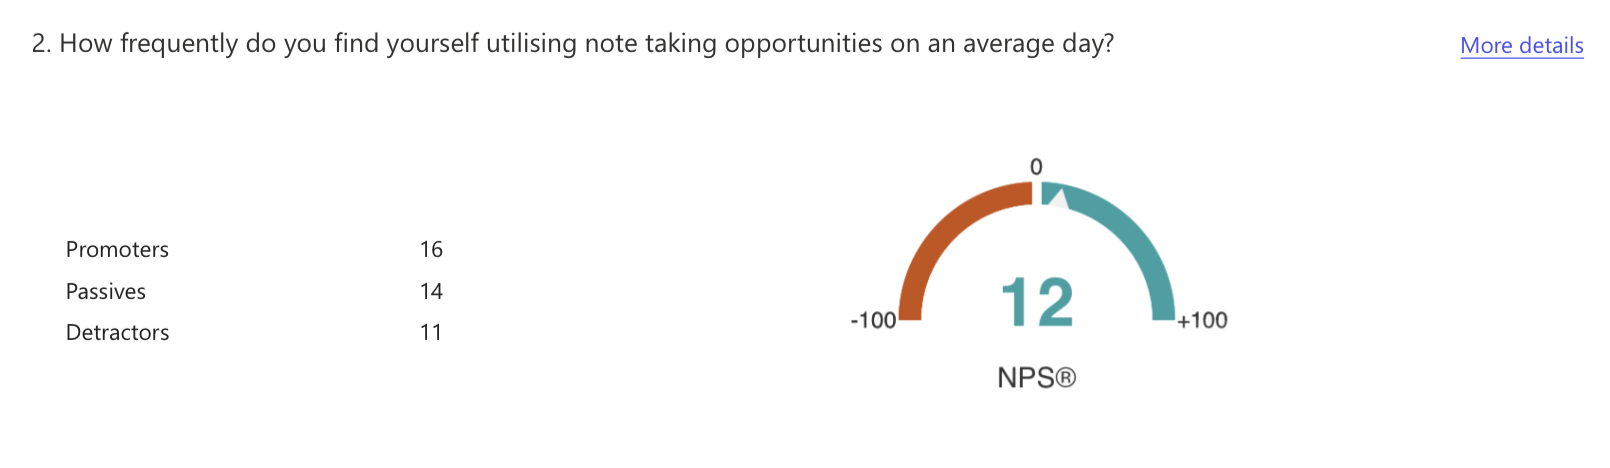
\includegraphics[width=0.8\textwidth]{Research/15_SurveyAnalysis/media/q2.png}
    \caption{Q2 responses}
\end{figure}
This question asked respondents to rank their use of note taking tool on a scale of 1-10 through a system called the net promoter score. To be Marked as a promoter respondents had to answer with a score of 9-10, passive a score of 7-8 and detractors from 6 and below. This scale aims to offset the natural instinct of humanity to tend to only tend to either extremes when they have an opinion, and those without will stay natural. Although this scale is objectively biased towards those who don’t use notes the results still ended positive which demonstrates a clear use of note taking tools among my respondents

\subsection*{Q3: Which devices do you use to take notes?}
\begin{figure}[H]
    \centering
    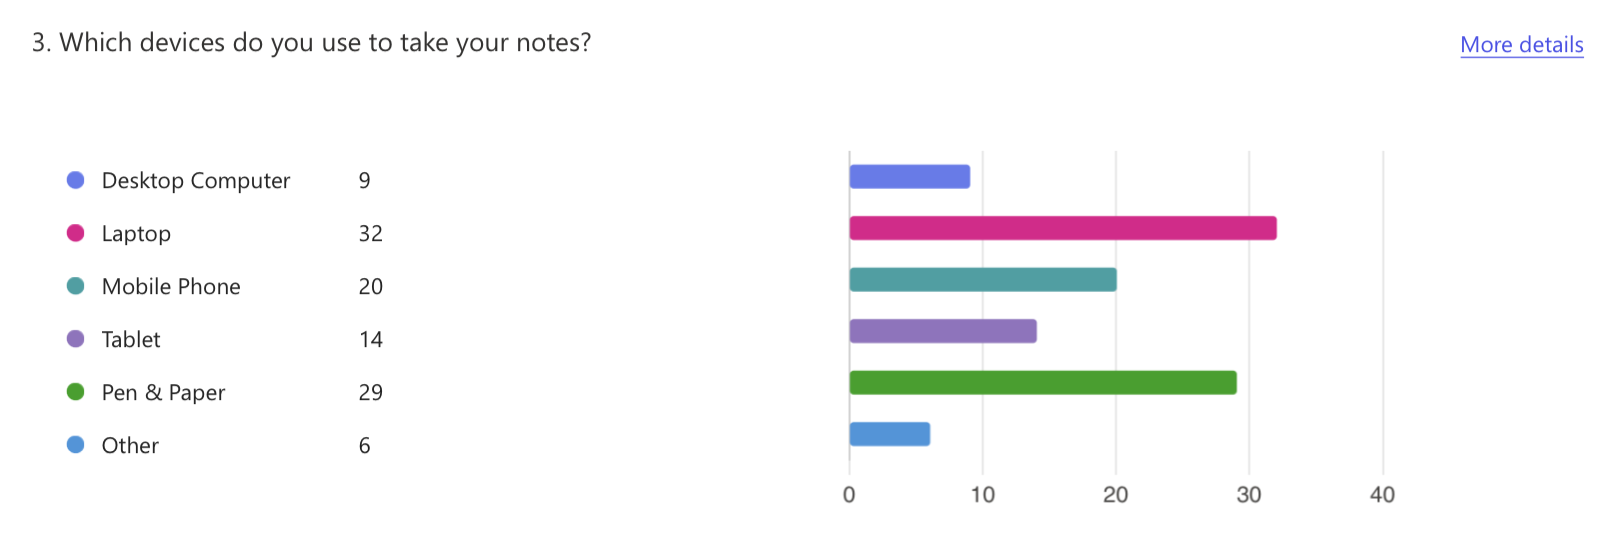
\includegraphics[width=0.8\textwidth]{Research/15_SurveyAnalysis/media/q3.png}
    \caption{Q3 responses}
\end{figure}
My third question asked respondents which devices they used to take notes. This was to help me inform which platforms I should target for releasing my application. As I had expected among my audience Laptop computers and mobile phones were the most used devices though a large number of respondents (58%) used traditional pen and paper, later on I found out why this was the case (and what digital provision was lacking). From this data I can see that it is important I ensure my artifact is well supported on both mobile devices and larger format computers, making touch interactivity a necessity. The other responses were (digital notebooks, smart wearables, and whiteboards) which all show the benefits my web approach will have towards less common smart devices like these

\subsection*{Q4: Do you use any of the following note taking tools?}
\begin{figure}[H]
    \centering
    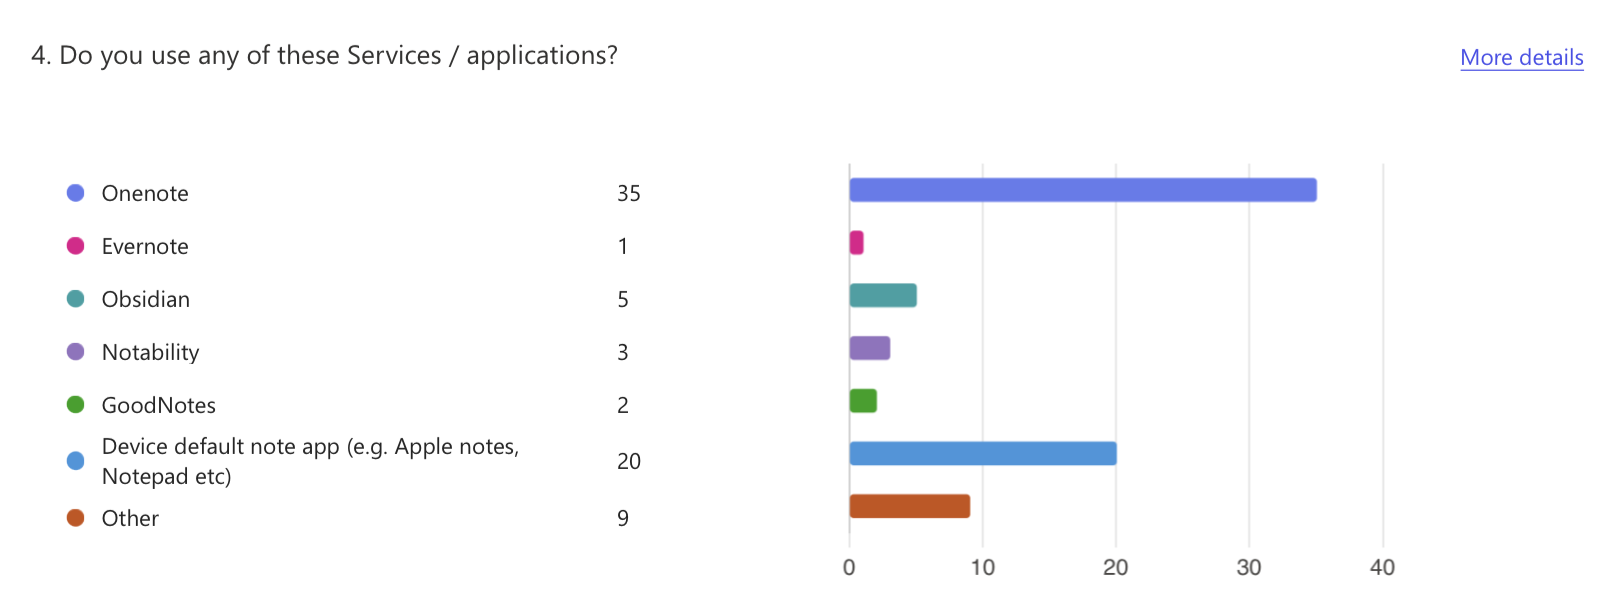
\includegraphics[width=0.8\textwidth]{Research/15_SurveyAnalysis/media/q4.png}
    \caption{Q4 responses}
\end{figure}
OneNote was clearly the dominant market leader among my peers which I would presume to be down to its strong interactivity with Microsoft teams enable teachers to share resources and synchronise work with their students. Whilst I cant match this interactivity I can explore creating some features (building off my previous research) to make syncing more seamless. The default note apps also saw some popularity (all other responses were considered defaults) among my respondents which is likely down to the ease of use and speed of making notes with a simple interface, I can learn a lot from this

\subsection*{Q5: Do you have any comments on the current note taking tools you use? What do you like and dislike about them}



\begin{longtable}{@{}p{0.47\textwidth}@{\hspace{1em}}p{0.47\textwidth}@{}}
\toprule
\textbf{Comment} & \textbf{Response} \\
\midrule
\endfirsthead

\toprule
\textbf{Comment} & \textbf{Response} \\
\midrule
\endhead

- I like syncing between devices. I like connectivity to outlook &
- Full device syncing is a pillar point of my brief and I can certainly explore outlook (email client) integration for sending email content to notes etc \\

- LIKE : Search function, cross platform, ease of use, voice dictation, transcription and summarisation with action points
 & - Voice transcription could also be explored as another input method \\

- excessive features, but then again lack of basic features such as erasing. & 
- Will ensure erasing is well implemented \\

- i wish device default note apps had a bit more functionality to them & 
- Hopefully my artifact should integrate these features\\ 

- I love the presentation and organization of notes in Obsidian, particularly in linking notes together. & 
- Obsidian is a huge inspiration for my 'node' layout and hopefully my artifact will only improve on this \\ 

- Like being able to resize my writing and move things around with ease; don't like how difficult it can be to select all the things I want. Also when writing on documents that have been printed onto OneNote, to stop selecting them continuously while writing, I have to select them all and set them as a background - would be nice to be able to do that more easily & 
- In my whiteboard view everything can be moved with ease, will also include layer 'locking' which fixes this issue \\ 

- occasional glitches or like the stylus doesn't draw despite working on other apps & 
- I will thoroughly test this among a variety of devices I have available, and ask peers to do the same on others \\ 

- Can't easily do maths in them & 
- Whiteboard like mode should enable easy writing for maths. Could also explore adding an inbuilt calculator tool\\ 

- I like how OneNote and the notes app are simple/easy to use &
- Hopefully i'll match that success \\ 

- lack of a ruler on OneNote, process of deleting pages and sections on OneNote and lack of clarity within this, differences in the software across devices with different operating systems and devices & 
- I can certainly explore adding a ruler (for measurement and straight line drawing), deleting files will be done in a clear way to prevent mistakes and as a web-app the software should appear very similar among devices \\ 

- Difficult to type complex formula & 
- By adding 'markdown' support this will be improved hugely \\ 

- I like easy formatting  & \\ 


- Moving text around pictures is hard & 
- I'm already planning to diverge away from Microsoft default text wrapping approach which should solve this \\ 

- I like how simple it is to use the option pad & 
- Not quire sure what the 'option pad' is but I'm aiming to make controls customisable \\

- When bullet points don't behave like they normally do. & 
- I'm aiming to follow the standard approach for bullet points which should address this \\ 

- General functionality, the new one note is annoying because it randomly selects all the drawings and photos. & \\

- Can’t use inking on notion & 
- One huge downside of notion which I am fixing  \\

- I enjoy the graph views provided by Obsidian, and the use of markdown makes formatting easy. & 
- Again, my graph view is inspired by obsidian and am already working towards a markdown like approach to formatting more rigid documents \\
 
Having an unlimited area to write on a page & 
Am already building an 'infinite' size of workspace that can be panned and zoomed around\\

- Notability is so much better than OneNote. OneNote is laggy, has less features and is a lot less creative than notability  & 
- Clearly a user who prefers the notability approach to working and hopefully will enjoy using my artefact\\

- I like how notion and obsidian offer a way to easily link between pages. Also the ability to work real time collaboratively in some of the apps is really useful.  & 
- Powerful and flexible looping is already a key point of my project \\ 

- I like how easy it is to format using markdown and think that gives me a lot of opportunity. I dislike how I can't use digital inking.& 
see above \\ 

- Unlimited space on OneNote makes it difficult when converting to PDF as you don’t know where the page boundary is. & 
- This is an interesting point that is common with infinite whiteboards, I could explore adding 'bounds' whilst exporting to help tidy up document though this might be outside the scope of my project \\ 

- It would be nice if it was less easy to accidentally delete things on OneNote & 
- Will ensure note deletions require at least two interactions, e.g. are you sure you want to delete this note? \\ 

- I like that OneNote is really easy to type and draw wherever you want, and its nice and organised, good that its not limited to separate pages (nice and continuous), but its so SLOW &
-  The flexible writing will be well supported in my program, and as a modern webapp there should be no performance concerns \\ 

- On the iPad version of OneNote it's a hassle to move pages and the layout is less accessible compared to the windows version, especially in terms of viewing the side tabs and sections. In OneNote there are sometimes also issues with features like ink to shape and when using the inbuilt shape tool e.g. you can only draw one shape at a time meaning you have to keep clicking on the shapes icon (rather than it staying in shape-drawing mode until you click off it) & 
- See above, this feedback might also mean me adding a option lock command which allows the user to keep executing the  command until unlocked (e.g. adding shapes until the esc key is pressed) \\

- Syncing issues especially on pages with many not (presumably notes) & 
- See above \\

\bottomrule
\end{longtable}


\subsection*{Q6: Do you use any of these note-taking techniques?}
\begin{figure}[H]
    \centering
    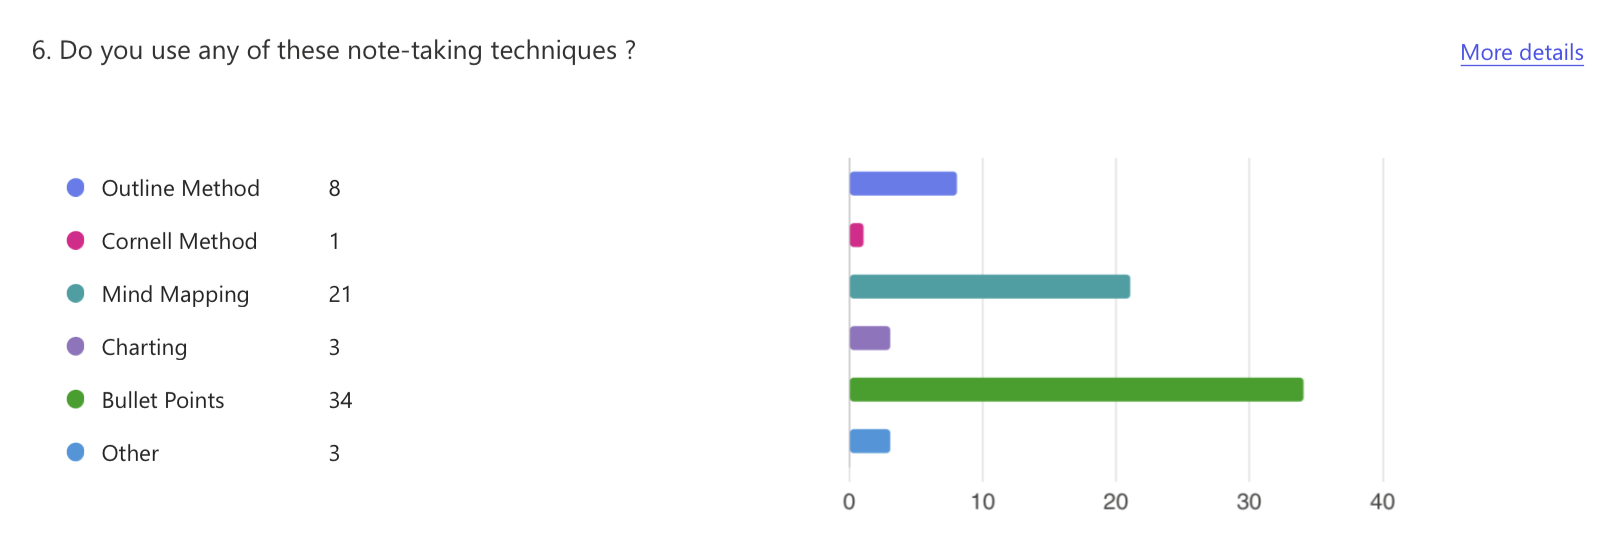
\includegraphics[width=0.8\textwidth]{Research/15_SurveyAnalysis/media/q6.png}
    \caption{Q6 responses}
\end{figure}
OneNote was clearly the dominant market leader among my peers which I would presume to be down to its strong interactivity with Microsoft teams enable teachers to share resources and synchronise work with their students. Whilst I cant match this interactivity I can explore creating some features (building off my previous research) to make syncing more seamless. The default note apps also saw some popularity (all other responses were considered defaults) among my respondents which is likely down to the ease of use and speed of making notes with a simple interface, I can learn a lot from this

\subsection*{Q7: Which of these styles of notes do you use?}
\begin{figure}[H]
    \centering
    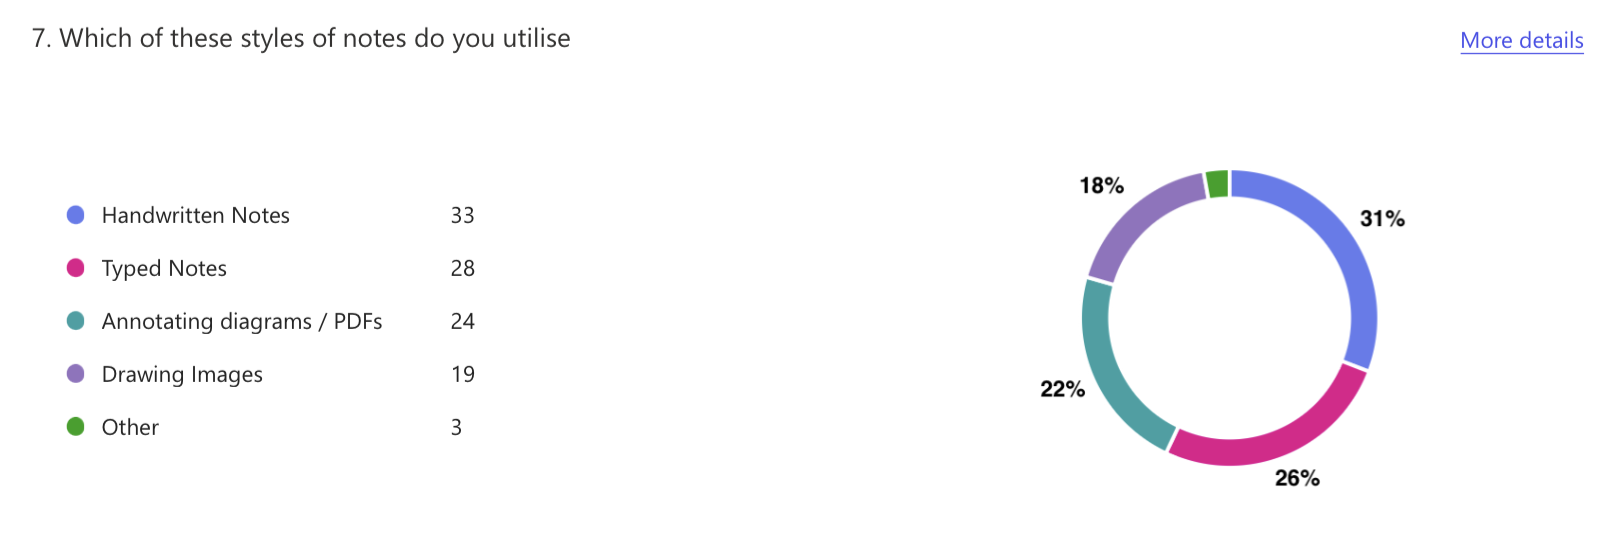
\includegraphics[width=0.8\textwidth]{Research/15_SurveyAnalysis/media/q7.png}
    \caption{Q7 responses}
\end{figure}
Further breaking down the style of notes used I found handwriting to narrowly lead out typed notes. It must therefore be prioritised in my development time spent. As I discovered in my research on academic papers surrounding the subject, handwriting has many benefits to information retention. Whilst handwriting is most used, typing is still incredibly important especially for quick (e.g. during lecture) note taking and I want to explore techniques used for formatting fully typed documents such as markup (a term I am already familiar with)


\subsection*{Q8: Please rank how important the following features are to you when using note taking tools}
\begin{figure}[H]
    \centering
    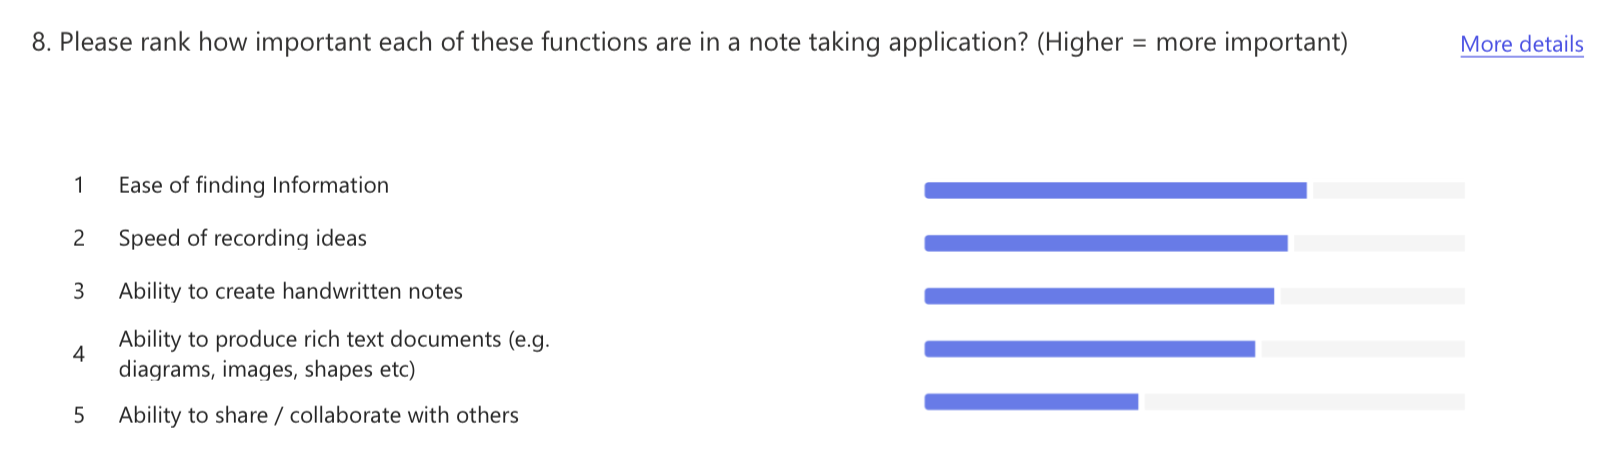
\includegraphics[width=0.8\textwidth]{Research/15_SurveyAnalysis/media/q8.png}
    \caption{Q8 responses}
\end{figure}
Further breaking down the style of notes used I found handwriting to narrowly lead out typed notes. It must therefore be prioritised in my development time spent. As I discovered in my research on academic papers surrounding the subject, handwriting has many benefits to information retention. Whilst handwriting is most used, typing is still incredibly important especially for quick (e.g. during lecture) note taking and I want to explore techniques used for formatting fully typed documents such as markup (a term I am already familiar with)


\subsection*{Q9: which information retrieval techniques do you believe is most efficent?}
\begin{figure}[H]
    \centering
    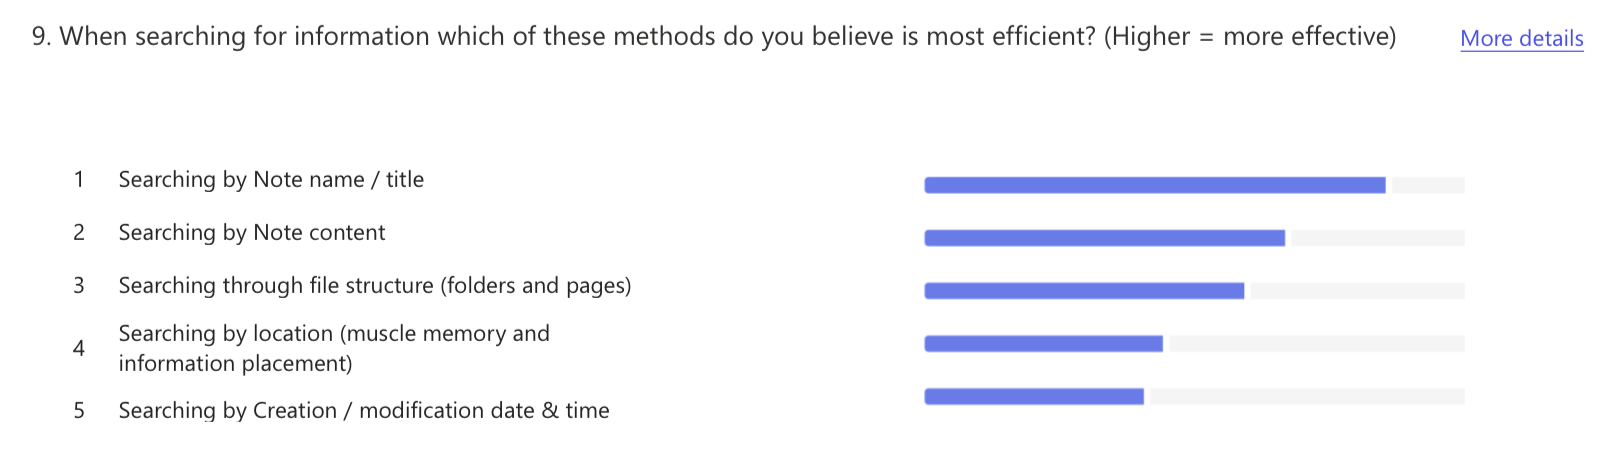
\includegraphics[width=0.8\textwidth]{Research/15_SurveyAnalysis/media/q9.png}
    \caption{Q9 responses}
\end{figure}
This question aims to ascertain the methods of sorting / finding my users use for data retrieval and the data gathered largely mirrors my expectations. I was expecting my younger user base to be primarily familiar with digital note taking systems which often use a folder-> child architecture. For these digital systems finding content by name and content is usually easiest to develop hence why it is so commonly seen in platforms such as OneNote. My usage of graphic organisation techniques through nodes is largely unique as a primary searching format and will hopefully prove more effective than the more rigid structure of folders. These results also largely mirror the research papers I read on note location and the techniques used to help users find information, whilst searching by location and time is effective it can be hard to implement and must be carefully considered.


\subsection*{Q10: Open commentary}

\begin{longtable}{@{}p{0.47\textwidth}@{\hspace{1em}}p{0.47\textwidth}@{}}
\toprule
\textbf{Comment} & \textbf{Response} \\
\midrule
\endfirsthead

\toprule
\textbf{Comment} & \textbf{Response} \\
\midrule
\endhead


- Linking of content between separate notes such that I can drill down on a topic. &
- Already a central feature \\

- For me it is all about ease of use and ease of accessing the information when I want it (assuming security and other essential features are all a given).  &
- Will ensure these are my focus points \\

- no it'll be great &
- A sign of confidence :) \\

- Possibly further options in permissions when sharing notes? E.g. some people have permissions to write and draw, while others only have permission to write &
- Very interesting and I can definitely explore. I find current systems often lack flexibility even down to letting others edit one area of text but not another \\

- Still being able to swap between pens whilst having a full screen for writing &
- Will ensure I retain this during my UI design \\

 - a motion to use eraser function without having to keep clicking between draw and eraser function, same with other functions &
 - I am not sure on the technical feasibility of this but will definitely explore and if possible to add reliably make it an option for users (I can see some maybe not wanting this by default) \\

 - easy maths tool & 
 - Not quite sure what this entails but as mentioned above I can explore adding tools such as automatic graph drawing and calculation solving \\

 - Please make it less resource intensive than OneNote (not very hard) &
 - Web based applications are fundamentally lighter than desktop apps so this should be achieved \\

 - Ease of use with complex formula. Maybe having presets for easy commands so for chemistry I have lots of symbols without sub menus &
 - Another very interesting point for a non standard workflow, this would likely be another feature I would make optional but I can certainly see this being useful and saving time for users \\

 - Have multiple pages open at once. eg: in OneNote i could either switch between two pages of economics or have them appear next to each other without having to use two windows &
 - I can certainly explore multi-tab interfaces to enable side-by-side collaboration on documents, I can also see this being extended to enable viewing of the overall graph whilst a documents is being edited, I will certainly explore further \\

 - Tabs to take me to different sections within the page &
 - This sounds almost like a contents page within each note (possibly useful for longer form factor notes) which I can add \\

 - Take watermarks off images, zoom easily, search handwritten notes &
 - The first point is likely a legally and ethically dubious feature and so I will likely avoid this however searching of handwritten notes through tools such as OCR is ambitious but certainly on my radar \\

 - If I could mentally write notes that would be helpful &
 - Unfortunately not possible with todays technology \\

 - I feel like a node based system to connect different notes would really aid in representing the way my mind links different ideas. &
 - Exactly what I am creating so my artifact sounds like a perfect solution to this persons needs \\

 - A good system for working with written notes but still has the ability to create networks of notes. &
 - Similar to above, should be seamless :) \\

 - easy to insert images to annotate &
 Mentioned previously but will definitely be added \\

 - Good to be able to have a really thin pen, different colours, NOT SLOW. It’s also nice to be able to zoom out loads. Would be good to also have size options for the rubber where it just deletes chunks at a time (‘stroke’ rubber on OneNote), it’s annoying that the pen to select things on OneNote is so inaccurate and selects way more or way less than I want &
 - Whilst I don’t intend for this to be a platform designed for artwork I can add pen customisation easily. Same goes for the rubber where I can build options for 'stroke erasing' (which many people - me included, find easiest for deleted handwriting mistakes) and 'area' erasing (where parts of strokes are deleted) \\

 - I think this exists already in some applications but it would be nice if this was more widespread: feature where you can cover up/uncover some notes for revision/active recall purposes &
 - Another interesting feature to explore as a revision resource, and alongside many others is a stretch goal for me to aid not just the recording of information but the learning of it as well \\

\bottomrule
\end{longtable}

\subsection*{Contact}
Lastly I asked each respondent if they would like to provide an email address to receive updates when I have finished development of my later prototypes and am ready for reviews. Whilst completely optional to fill in (and the steps for me to remove these details made clear) I received 20 peoples contact details and look forward to conversing with them in a few months time to gain their crucial feedback once they can be hands on with my artifact

\subsection*{Feedback}
It also seems my thought to making the survey simple to fill in was appreciated by respondents having received this feedback and offers for even greater assistance:

\begin{quote}
    "That was actually really nice to fill in"
\end{quote}

\begin{quote}
    "I wish other surveys followed the same approach"
\end{quote}

\begin{figure}[H]
    \centering
    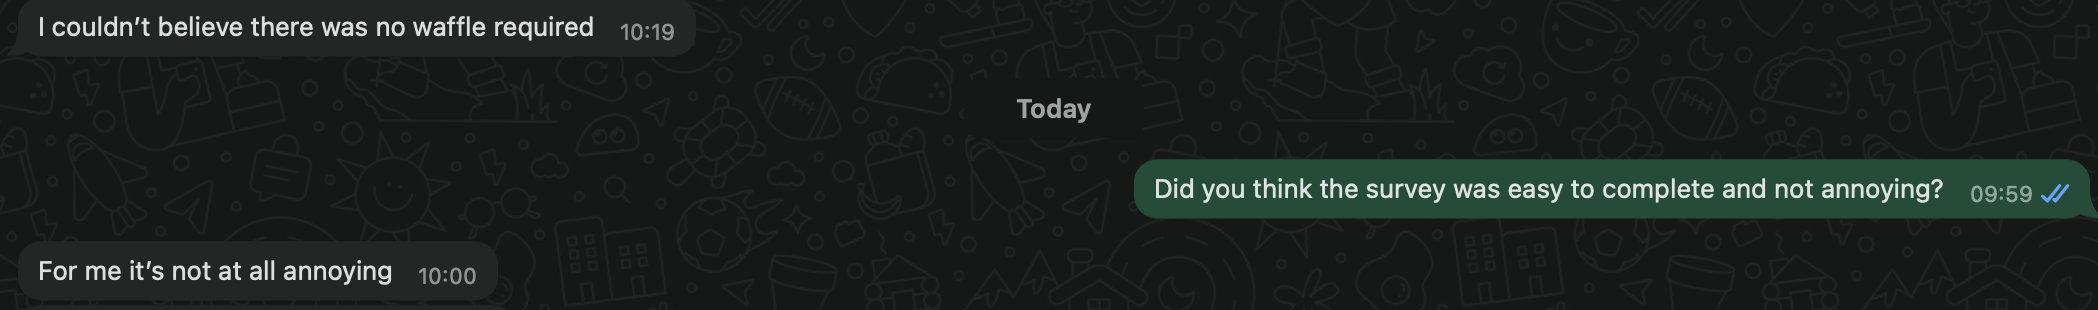
\includegraphics[width=0.8\textwidth]{Research/15_SurveyAnalysis/media/feedback1.png}
    \caption{feedback from respondents }
\end{figure}

\begin{figure}[H]
    \centering
    
\includegraphics[width=0.8\textwidth]{Research/15_SurveyAnalysis/media/feedback2.png}
    \caption{feedback from respondents }
\end{figure}

\begin{figure}[H]
    \centering
    
\includegraphics[width=0.8\textwidth]{Research/15_SurveyAnalysis/media/feedback3.png}
    \caption{feedback from respondents }
\end{figure}

